% contribution-no-refs.tex

% !TEX program = pdflatex
\documentclass[tikz]{standalone}
\usetikzlibrary{positioning, calc, arrows, arrows.meta, fit}

\newcommand{\jupiter}{\textsl{Jupiter}}
\newcommand{\cjupiter}{\textsl{CJupiter}}
\newcommand{\xjupiter}{\textsl{XJupiter}}
\newcommand{\ajupiter}{\textsl{AJupiter}}
\newcommand{\absjupiter}{\textsl{AbsJupiter}}
\newcommand{\wlspec}{\textsl{WLSpec}}
\renewcommand{\sec}{\textsl{SEC}}

\begin{document}
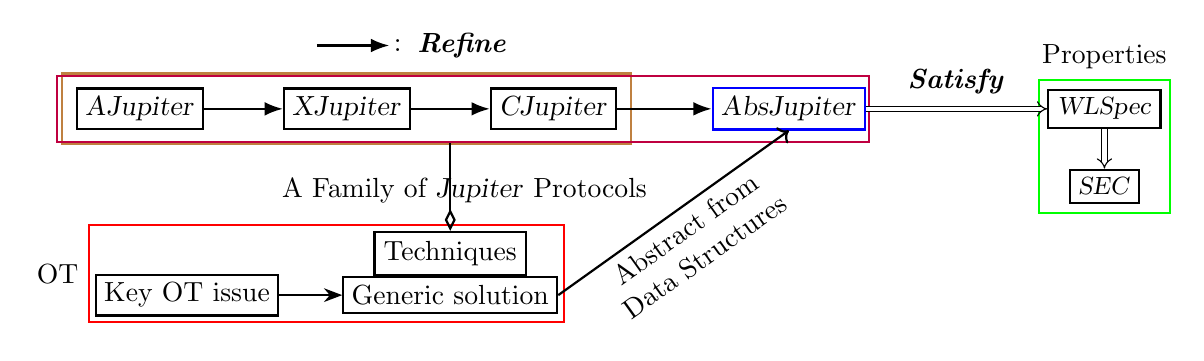
\begin{tikzpicture}[protocol/.style = {draw, thick, inner sep = 3pt},
  ot/.style = {draw, thick, inner sep = 3pt},
  st/.style = {-To, thick},
  spec/.style = {draw, thick, inner sep = 3pt},
  sat/.style = {double equal sign distance, -Implies},
  refine/.style = {>=LaTeX, ->, thick}]
  % jupiter protocols
  \node (aj) [protocol] {\ajupiter};
  \node (xj) [protocol, right = of aj] {\xjupiter};
  \node (cj) [protocol, right = of xj] {\cjupiter};

  % existing protocols: jupiter variants
  \node (jv) [draw, thick, brown, fit = (aj) (xj) (cj), inner sep = 5pt] {};

  % absjupiter
  \node (absj) [protocol, draw = blue, right = 1.2cm of cj, align = center]{\absjupiter};

  % jupiter family
  \node (ajabsj) at ($(aj)!0.5!(absj)$) {};
  \node (jflbl) [below = 18pt of ajabsj] {A Family of \jupiter{} Protocols};
  \node (jf) [draw, purple, thick, fit = (aj) (absj), xshift = -3pt, inner sep = 4pt] {};

  % ot
  \node (xcj) at ($(xj)!0.5!(cj)$) {};
  \node (sol) [ot, below = 2.0cm of xcj] {Generic solution};
  \node (issue) [ot, left = 0.80cm of sol]  {Key OT issue};

  \draw[-Stealth, thick] (issue) to (sol);

  \node (st) [draw, thick, above = 0.00cm of sol] {Techniques};
  \node (ot) [draw, thick, red, fit = (issue) (sol) (st), inner sep = 2pt, 
	label = {left : OT}] {};
  \draw[{Diamond[open]}-, thick] (st) to (jf.south -| st.north);

  % ot to absjupiter
  \draw[st] (sol.east) to node [below, sloped, align = center] 
    {Abstract from \\ Data Structures} (absj.south);

  % refine
  \path (aj) edge[refine] node (ajrefinexj) {} (xj)
		(xj) edge[refine] node (xjrefinecj) {} (cj)
		(cj) edge[refine] node (cjrefineabsj) {} (absj);
  \node (refinement) [above = 4pt of jf, inner sep = 2pt, label = {left: $:$}] 
    {\textbf{\emph{Refine}}};
  \draw[refine, shorten >= 8pt] ($(refinement.west)+(-1.2cm, 0)$) to (refinement);

  % specs
  \node (wlspec) [spec, right = 2.30cm of absj, align = center] {{\small \wlspec}};
  \node (sec) [spec, below = 0.50cm of wlspec] {{\small \sec}};
  \node (spec) [fit = (wlspec) (sec), draw, green, thick, inner sep = 3pt, 
    label = above : Properties] {};

  \draw [sat] (absj) to node [above = 2pt] {\textbf{\emph{Satisfy}}} (wlspec);
  \path (wlspec) edge[sat] (sec);
\end{tikzpicture}
\end{document}